\documentclass[11pt,a4paper]{article}

\usepackage[utf8]{inputenc}
\usepackage[T1]{fontenc}
\usepackage{lmodern}
\usepackage[margin=1in]{geometry}
\usepackage{hyperref}
\usepackage{booktabs}
\usepackage{longtable}
\usepackage{xcolor}
\usepackage{listings}
\usepackage{enumitem}
\usepackage{tikz}
\usetikzlibrary{shapes.geometric, arrows.meta, positioning}

\hypersetup{
  colorlinks=true,
  linkcolor=blue!60!black,
  urlcolor=blue!60!black,
  pdftitle={Codefied Technical Documentation},
  pdfauthor={Codefied Engineering}
}

\definecolor{codebg}{RGB}{245,245,245}
\definecolor{codeframe}{RGB}{200,200,200}

\lstdefinestyle{terminal}{
  backgroundcolor=\color{codebg},
  frame=single,
  rulecolor=\color{codeframe},
  basicstyle=\ttfamily\small,
  breaklines=true,
  columns=fullflexible,
  showstringspaces=false
}

\lstdefinestyle{envfile}{
  backgroundcolor=\color{codebg},
  frame=single,
  rulecolor=\color{codeframe},
  basicstyle=\ttfamily\small,
  breaklines=true
}

\newcommand{\maskedvercel}{\texttt{https://codefied-****.vercel.app}}
\newcommand{\maskedecip}{\texttt{54.166.**.53}}
\newcommand{\maskedrepo}{\texttt{github.com/[REDACTED]/Codefied}}

\title{\textbf{Codefied --- Technical Documentation}}
\author{Engineering Reference}
\date{July 2026}

\begin{document}
\maketitle
\tableofcontents
\newpage

\section{Project Overview}

\textbf{Codefied} is a full-stack online judge platform consisting of:
\begin{itemize}[noitemsep]
  \item A React SPA frontend (Vite + Tailwind), hosted on Vercel.
  \item An Express REST API managed by \textbf{PM2} on AWS EC2 (not a Docker container in production).
  \item \textbf{nginx} on EC2 (:80) reverse-proxying to the Node process on :4000.
  \item A sandboxed code execution engine (C/C++/Java/Python) using host-installed compilers.
  \item MongoDB Atlas for persistent data.
  \item Redis 7 (Docker, \texttt{127.0.0.1:6379} only) for AI review rate limiting.
  \item Google Gemini for synchronous AI code review.
\end{itemize}

\textbf{Repository:} \maskedrepo

\section{Technology Stack}

\subsection{Frontend}
\begin{table}[h]
\centering
\small
\begin{tabular}{@{}lll@{}}
\toprule
\textbf{Technology} & \textbf{Version} & \textbf{Purpose} \\
\midrule
React               & 19.x   & UI framework \\
Vite                & 8.x    & Build tool and dev server \\
React Router DOM    & 7.x    & Client-side routing \\
Tailwind CSS        & 4.x    & Utility-first styling \\
@tailwindcss/vite   & 4.x    & Tailwind Vite integration \\
@monaco-editor/react& 4.x    & \texttt{CodeEditor} component \\
Axios               & 1.x    & HTTP client (\texttt{withCredentials}) \\
react-markdown      & 10.x   & Render problem descriptions and AI output \\
esbuild             & 0.28.x & Vite production transpilation \\
\bottomrule
\end{tabular}
\end{table}

\subsection{Backend}
\begin{table}[h]
\centering
\small
\begin{tabular}{@{}lll@{}}
\toprule
\textbf{Technology} & \textbf{Version} & \textbf{Purpose} \\
\midrule
Node.js             & 20.x   & Runtime (PM2 on EC2 host) \\
Express             & 5.x    & HTTP API framework \\
Mongoose            & 9.x    & MongoDB ODM \\
bcryptjs            & 3.x    & Password hashing \\
jsonwebtoken        & 9.x    & JWT access/refresh tokens \\
cookie-parser       & 1.x    & HTTP-only auth cookies \\
cors                & 2.x    & Cross-origin policy \\
dotenv              & 17.x   & Environment configuration \\
ioredis + redis     & 5.x/6.x& Redis client (rate limiting) \\
@google/genai       & 2.x    & Gemini API SDK \\
uuid                & 14.x   & Sandbox job IDs \\
slugify             & 1.x    & Problem slug generation \\
PM2                 & latest & Process manager on EC2 \\
\bottomrule
\end{tabular}
\end{table}

\textbf{Note:} \texttt{BullMQ} and \texttt{backend/jobs/aiReviewJob.js} exist for optional local/queue-based development but are \textbf{not used in production}. AI review is invoked synchronously via \texttt{aiCodereview()}.

\subsection{Infrastructure and DevOps}
\begin{table}[h]
\centering
\small
\begin{tabular}{@{}ll@{}}
\toprule
\textbf{Tool / Service} & \textbf{Role} \\
\midrule
Vercel                  & Frontend hosting, HTTPS, SPA routing, \texttt{/api} proxy to EC2 \\
AWS EC2 t3.small (Amazon Linux 2023) & Backend compute, nginx, PM2, host compilers \\
AWS Elastic IP          & Static EC2 public address (\maskedecip) \\
nginx                   & Reverse proxy :80 $\rightarrow$ \texttt{127.0.0.1:4000} \\
PM2                     & Keeps \texttt{codefied-api} alive; memory cap 450\,MB \\
Docker + Docker Compose & Redis container only in production \\
Redis 7 (Alpine image)  & Rate-limit store (\texttt{127.0.0.1:6379}) \\
MongoDB Atlas M0        & Managed database \\
GitHub                  & Source control \\
OpenSSH                 & EC2 administration \\
\bottomrule
\end{tabular}
\end{table}

\subsection{Compiler Runtimes (EC2 Host)}
Installed on the EC2 host via \texttt{dnf} (see \texttt{scripts/setup-t3-small.sh}):
\begin{itemize}[noitemsep]
  \item \texttt{gcc}, \texttt{gcc-c++} --- C and C++
  \item \texttt{python3} --- Python
  \item \texttt{java-21-amazon-corretto-devel} --- Java (\texttt{javac}, \texttt{java})
\end{itemize}

An optional \texttt{backend/Dockerfile} image (profile \texttt{docker} in Compose) bundles the same compilers for local Docker-based development; production does \textbf{not} run the backend in Docker.

\section{System Architecture}

\begin{center}
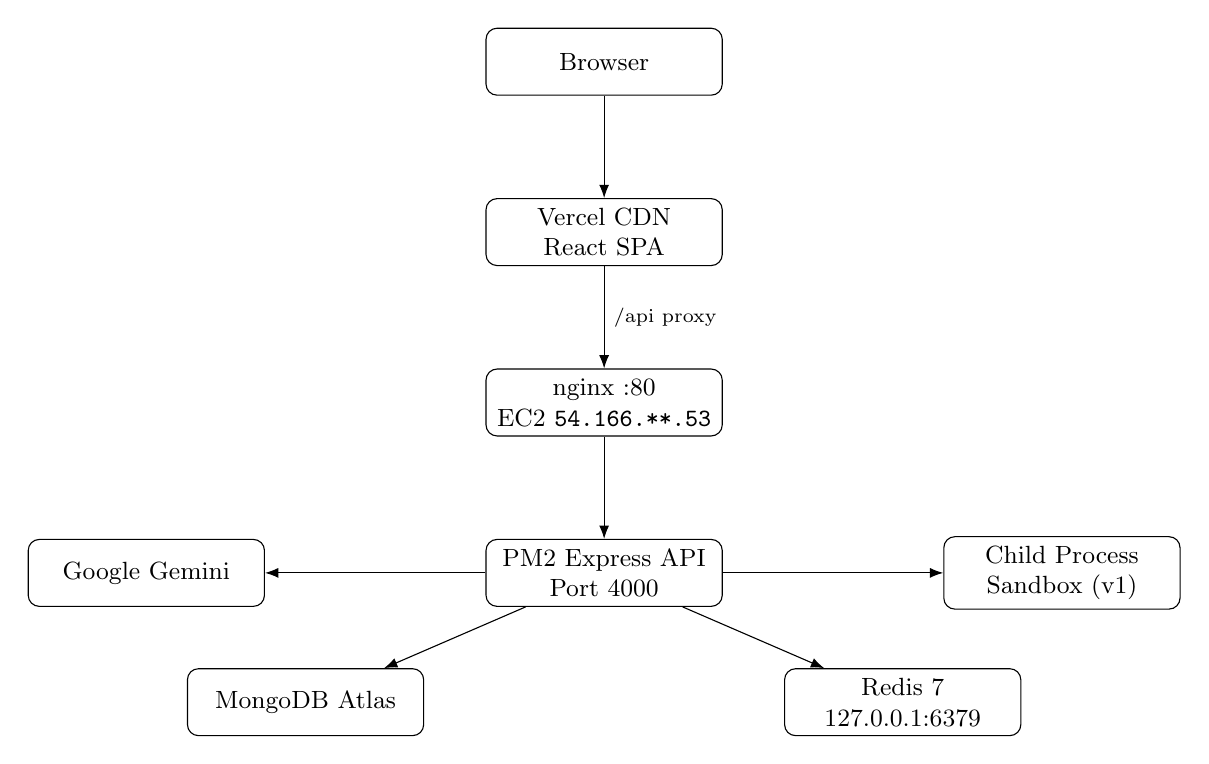
\begin{tikzpicture}[
  node distance=1.3cm,
  box/.style={draw, rounded corners, minimum width=3cm, minimum height=0.85cm, align=center, font=\small}
]
  \node[box] (browser) {Browser};
  \node[box, below=of browser] (vercel) {Vercel CDN\\React SPA};
  \node[box, below=of vercel] (nginx) {nginx :80\\EC2 \maskedecip};
  \node[box, below=of nginx] (api) {PM2 Express API\\Port 4000};
  \node[box, below left=1.1cm of api] (mongo) {MongoDB Atlas};
  \node[box, below right=1.1cm of api] (redis) {Redis 7\\127.0.0.1:6379};
  \node[box, right=2.8cm of api] (sandbox) {Child Process\\Sandbox (v1)};
  \node[box, left=2.8cm of api] (gemini) {Google Gemini};

  \draw[-{Latex}] (browser) -- (vercel);
  \draw[-{Latex}] (vercel) -- node[right, font=\scriptsize]{/api proxy} (nginx);
  \draw[-{Latex}] (nginx) -- (api);
  \draw[-{Latex}] (api) -- (mongo);
  \draw[-{Latex}] (api) -- (redis);
  \draw[-{Latex}] (api) -- (gemini);
  \draw[-{Latex}] (api) -- (sandbox);
\end{tikzpicture}
\end{center}

\subsection{Production vs.\ Local Development}
\begin{table}[h]
\centering
\small
\begin{tabular}{@{}lll@{}}
\toprule
\textbf{Component} & \textbf{Production (EC2)} & \textbf{Local Dev} \\
\midrule
Backend runtime    & PM2 + host Node.js        & \texttt{node server.js} or Docker profile \\
Redis              & Docker, localhost bind    & Docker Compose \\
Compilers          & Host packages             & Host or Docker image \\
API ingress        & nginx :80                 & Direct :4000 \\
Frontend API URL   & \texttt{/api} (Vercel proxy) & \texttt{http://localhost:4000/api} \\
\bottomrule
\end{tabular}
\end{table}

\subsection{Request Flow (Authenticated API Call)}
\begin{enumerate}[noitemsep]
  \item Frontend Axios instance sends request to \texttt{/api/...} (Vercel same-origin).
  \item Vercel rewrites to \texttt{http://\maskedecip/api/...} (nginx on EC2).
  \item nginx proxies to \texttt{127.0.0.1:4000}.
  \item Express CORS checks \texttt{FRONTEND\_URL}; \texttt{credentials: true} allows cookies.
  \item \texttt{auth} middleware verifies JWT from \texttt{accessToken} HTTP-only cookie (Bearer header accepted as fallback).
  \item Controller executes business logic; MongoDB/Redis/sandbox engaged as needed.
  \item JSON response returned through nginx and Vercel to browser.
  \item On 401, Axios interceptor calls \texttt{POST /api/auth/refresh} and retries the original request.
\end{enumerate}

\section{Repository Structure}

\begin{lstlisting}[style=terminal]
OC/
|-- frontend/                      # React SPA (Vercel root)
|   |-- src/
|   |   |-- pages/                 # Route pages incl. SubmissionsPage
|   |   |-- components/            # Navbar, ProtectedRoute, CodeEditor
|   |   |-- context/               # AuthContext (cookie session)
|   |   |-- services/api.js        # Axios + refresh interceptor
|   |-- vercel.json                # SPA + /api proxy to EC2
|   |-- vite.config.js
|   `-- package.json
|-- backend/
|   |-- index.js                   # Express app entry (dotenv, routes)
|   |-- server.js                  # Requires index.js (PM2 entry)
|   |-- ecosystem.config.cjs       # PM2 process definition
|   |-- executeCode.js             # v1 sandbox runner
|   |-- aiCodereview.js            # Direct Gemini integration
|   |-- controllers/               # Route handlers
|   |-- routes/                    # API routers
|   |-- models/                    # Mongoose schemas
|   |-- middleware/                # auth (JWT-only), rateLimit
|   |-- jobs/aiReviewJob.js        # Optional BullMQ (not production)
|   |-- utils/                     # jwt, redis, cookies, verdict, solvedStats
|   |-- config/db.js
|   |-- scripts/seedProblems.js
|   `-- Dockerfile                 # Optional local Docker backend
|-- deploy/
|   `-- nginx/
|       `-- codefied.conf          # :80 -> :4000 reverse proxy
|-- scripts/
|   |-- setup-t3-small.sh          # Full EC2 production bootstrap
|   |-- preflight-ec2.sh           # Health checks before/after deploy
|   |-- ec2-optimize.sh            # Swap + memory tuning
|   `-- fix-services.sh            # Restart nginx/PM2/Redis
|-- docker-compose.yml             # Redis (+ optional docker backend profile)
|-- .env                           # Repo-root env (PM2 loads via ../.env)
|-- DEPLOYMENT.tex
|-- USER_MANUAL.tex
`-- TECHNICAL_DOCUMENTATION.tex
\end{lstlisting}

\section{Database Schema}

\subsection{User}
\begin{lstlisting}[style=envfile]
handle: String (unique, required)
email: String (unique, required)
passwordHash: String (required, bcrypt)
role: String (default: "user")
tokenVersion: Number (default: 0)
timestamps: createdAt, updatedAt
\end{lstlisting}

\subsection{Problem}
\begin{lstlisting}[style=envfile]
title, slug (unique), description (Markdown)
difficulty: enum [easy, medium, hard]
constraints, timeLimit (ms), memoryLimit (MB)
tags: [String]
sampleCases: [{ input, expectedOutput }]
sampleInput, sampleOutput, starterCode (legacy fields)
createdBy: ObjectId -> User
\end{lstlisting}

\subsection{TestCase (Hidden)}
\begin{lstlisting}[style=envfile]
problemId: ObjectId -> Problem
input, expectedOutput: String
isHidden: Boolean (true for judge cases)
order: Number
\end{lstlisting}

\subsection{Submission}
\begin{lstlisting}[style=envfile]
userId, problemId: ObjectId
code, language: String
verdict: pending | accepted | wrong-answer
         | time-limit-exceeded | compile-error | runtime-error
runtime, memory: Number
results: Array (per-test-case detail with verdict per case)
timestamps
\end{lstlisting}

Verdict resolution is centralized in \texttt{backend/utils/verdict.js} (\texttt{VERDICTS} enum, \texttt{resolveCaseVerdict}, \texttt{resolveSubmissionVerdict}).

\section{REST API Reference}

Base path: \texttt{/api}. All routes below are relative to that prefix.

\subsection{Authentication (\texttt{/api/auth})}
\begin{table}[h]
\centering
\small
\begin{tabular}{@{}lllp{4.5cm}@{}}
\toprule
\textbf{Method} & \textbf{Path} & \textbf{Auth} & \textbf{Description} \\
\midrule
POST & \texttt{/register} & No  & Create account; sets access + refresh cookies \\
POST & \texttt{/login}    & No  & Login; sets access + refresh cookies \\
POST & \texttt{/refresh}  & Cookie & Rotate access cookie from refresh cookie \\
POST & \texttt{/logout}   & No  & Clear both auth cookies \\
GET  & \texttt{/me}       & Yes & Current user + \texttt{solvedCount} \\
\bottomrule
\end{tabular}
\end{table}

\subsection{Problems (\texttt{/api/problems})}
\begin{table}[h]
\centering
\small
\begin{tabular}{@{}lllp{4.8cm}@{}}
\toprule
\textbf{Method} & \textbf{Path} & \textbf{Auth} & \textbf{Description} \\
\midrule
GET  & \texttt{/}     & Yes & List problems \\
GET  & \texttt{/:id}  & Yes & Problem detail + samples \\
POST & \texttt{/}     & Yes & Create problem + test cases \\
\bottomrule
\end{tabular}
\end{table}

\subsection{Submissions (\texttt{/api/submissions})}
\begin{table}[h]
\centering
\small
\begin{tabular}{@{}lllp{5cm}@{}}
\toprule
\textbf{Method} & \textbf{Path} & \textbf{Auth} & \textbf{Description} \\
\midrule
GET  & \texttt{/me}         & Yes & Paginated submission history for current user \\
GET  & \texttt{/me/:id}    & Yes & Single submission detail (includes code) \\
POST & \texttt{/run/:id}    & Yes & Run against sample cases \\
POST & \texttt{/submit/:id} & Yes & Judge against hidden cases; returns verdict enum \\
\bottomrule
\end{tabular}
\end{table}

\texttt{GET /me} supports query filters: \texttt{?problemId=}, \texttt{?verdict=}, \texttt{?page=}, \texttt{?limit=} (max 100).

\subsection{Users (\texttt{/api/users})}
\begin{table}[h]
\centering
\small
\begin{tabular}{@{}lllp{4.5cm}@{}}
\toprule
\textbf{Method} & \textbf{Path} & \textbf{Auth} & \textbf{Description} \\
\midrule
GET & \texttt{/me}          & Yes & Profile with solvedCount \\
GET & \texttt{/leaderboard} & Yes & Top 50 by unique solves \\
\bottomrule
\end{tabular}
\end{table}

\subsection{Compiler (\texttt{/api/compiler})}
\begin{table}[h]
\centering
\small
\begin{tabular}{@{}lllp{4.8cm}@{}}
\toprule
\textbf{Method} & \textbf{Path} & \textbf{Auth} & \textbf{Description} \\
\midrule
POST & \texttt{/run}      & No* & Execute code with custom input \\
POST & \texttt{/aiReview} & Yes & Synchronous Gemini review (rate limited) \\
\bottomrule
\end{tabular}
\caption{*Run is unauthenticated in router; called from authenticated frontend session}
\end{table}

\subsection{Health}
\begin{table}[h]
\centering
\small
\begin{tabular}{@{}lllp{5cm}@{}}
\toprule
\textbf{Method} & \textbf{Path} & \textbf{Auth} & \textbf{Description} \\
\midrule
GET & \texttt{/api/health} & No & Uptime and memory snapshot \\
\bottomrule
\end{tabular}
\end{table}

\section{Authentication Design}

\subsection{Token Model (Cookie-Only)}
\begin{itemize}[noitemsep]
  \item \textbf{Access token:} JWT, 15-minute expiry, HTTP-only cookie \texttt{accessToken}.
  \item \textbf{Refresh token:} JWT, 7-day expiry, HTTP-only cookie \texttt{refreshToken}.
  \item \textbf{No \texttt{localStorage}} --- tokens are never stored in browser storage.
  \item Axios is configured with \texttt{withCredentials: true} so cookies attach to every request.
  \item Response interceptor on 401 (non-auth routes) calls \texttt{POST /auth/refresh}, then retries the failed request.
  \item \texttt{AuthContext} restores session via \texttt{GET /auth/me}, falling back to refresh on failure.
\end{itemize}

\subsection{Auth Middleware (\texttt{backend/middleware/auth.js})}
\begin{itemize}[noitemsep]
  \item Reads \texttt{accessToken} from cookies; falls back to \texttt{Authorization: Bearer} header.
  \item Verifies JWT signature and expiry only --- \textbf{no database lookup per request}.
  \item Attaches \texttt{req.user} with \texttt{\_id}, \texttt{handle}, \texttt{role} from token claims.
  \item Refresh endpoint (\texttt{/auth/refresh}) is the only auth path that queries MongoDB (\texttt{tokenVersion} check).
\end{itemize}

\subsection{Cookie Policy (\texttt{backend/utils/cookies.js})}
\begin{itemize}[noitemsep]
  \item Both cookies: \texttt{httpOnly: true}, \texttt{path: /}.
  \item Local dev: \texttt{sameSite=lax}, \texttt{secure=false}.
  \item Production cross-origin (Vercel $\rightarrow$ EC2): \texttt{sameSite=none}, \texttt{secure=true} when \texttt{FRONTEND\_URL} is not localhost.
  \item Controlled via \texttt{COOKIE\_SECURE} and \texttt{FRONTEND\_URL} env vars.
\end{itemize}

\subsection{Environment Loading (\texttt{backend/index.js})}
PM2 runs with \texttt{cwd = backend/}. dotenv loads:
\begin{enumerate}[noitemsep]
  \item \texttt{../.env} --- repo-root file written by \texttt{setup-t3-small.sh}
  \item \texttt{.env} --- optional backend-local override
\end{enumerate}

\subsection{Protected Routes (Frontend)}
\texttt{ProtectedRoute} wrapper redirects unauthenticated users to \texttt{/login}.

\section{Solved Count and Leaderboard}

Implemented in \texttt{backend/utils/solvedStats.js}:
\begin{itemize}[noitemsep]
  \item \texttt{getSolvedProblemIds(userId)} --- \texttt{Submission.distinct("problemId", \{ userId, verdict: "accepted" \})}.
  \item \texttt{getSolvedCount(userId)} --- size of distinct problem IDs (not raw submission count).
  \item \texttt{getLeaderboard(limit)} --- aggregation grouping by \texttt{(userId, problemId)} before counting, ensuring one solve per problem per user.
\end{itemize}

\section{Code Execution Sandbox}

Implemented in \texttt{backend/executeCode.js}.

\subsection{Version Roadmap}
\begin{itemize}[noitemsep]
  \item \textbf{v1 (current):} Child processes spawned on the EC2 host in isolated temp directories under \texttt{os.tmpdir()/coderunner/}. Same OS namespace as the API process.
  \item \textbf{v2 (planned):} Per-submission Docker container isolation with cgroup memory/CPU limits and no host filesystem sharing.
\end{itemize}

\subsection{Process}
\begin{enumerate}[noitemsep]
  \item Generate UUID job ID; create temp dir under \texttt{os.tmpdir()/coderunner/}.
  \item Write source file (\texttt{main.c}, \texttt{main.cpp}, \texttt{Main.java}, \texttt{main.py}).
  \item Compile if needed (\texttt{g++}, \texttt{gcc}, \texttt{javac}) using host binaries.
  \item Spawn child process with stdin from user input; per-problem \texttt{timeLimit} from DB (default 1000\,ms).
  \item Collect stdout, stderr, exit code; enforce timeout.
  \item Delete temp directory (best-effort cleanup with retry on \texttt{EBUSY}).
\end{enumerate}

\subsection{Verdict Mapping}
Per-case verdicts from \texttt{verdict.js}: \texttt{accepted}, \texttt{wrong-answer}, \texttt{time-limit-exceeded}, \texttt{compile-error}, \texttt{runtime-error}. Submission verdict is \texttt{accepted} only if all cases pass; otherwise the first failing case verdict is returned.

\subsection{Security Notes}
\begin{itemize}[noitemsep]
  \item Per-execution isolated temp directory.
  \item No network isolation per child process (v2 containers would address this).
  \item Not suitable for untrusted public code execution without additional sandboxing.
  \item EC2 security group should \textbf{not} expose port 4000 publicly; nginx :80 only.
\end{itemize}

\section{AI Review}

\textbf{Production path} (no BullMQ worker):
\begin{enumerate}[noitemsep]
  \item \texttt{POST /api/compiler/aiReview} $\rightarrow$ \texttt{auth} + \texttt{aiReviewRateLimit}.
  \item Handler calls \texttt{aiCodereview(code)} directly $\rightarrow$ Gemini model \texttt{gemini-3.5-flash}.
  \item Markdown review text returned synchronously in \texttt{\{ aiReview: "..." \}}.
\end{enumerate}

\textbf{Rate limits:} 2/hour, 8/day per user (Redis counters in \texttt{middleware/rateLimit.js}; in-memory fallback if Redis unavailable).

\textbf{Legacy:} \texttt{backend/jobs/aiReviewJob.js} defines a BullMQ queue/worker for optional async processing but is not started in production PM2 configuration.

\section{Frontend Components and Routes}

\subsection{CodeEditor (\texttt{frontend/src/components/CodeEditor.jsx})}
Reusable Monaco wrapper used on \texttt{CoderunnerPage} and \texttt{ProblemDetailPage}:
\begin{itemize}[noitemsep]
  \item Dark theme (\texttt{vs-dark}), language mapping for C/C++/Java/Python.
  \item Editor options: line numbers, bracket colorization, auto-indent, suggestions.
  \item \texttt{automaticLayout: true} for responsive resizing.
\end{itemize}

\subsection{Frontend Routes}
\begin{table}[h]
\centering
\small
\begin{tabular}{@{}lll@{}}
\toprule
\textbf{Path} & \textbf{Component} & \textbf{Access} \\
\midrule
\texttt{/login} & LoginPage & Public \\
\texttt{/register} & RegisterPage & Public \\
\texttt{/dashboard} & DashboardPage & Auth \\
\texttt{/problems} & ProblemsPage & Auth \\
\texttt{/problems/:problemId} & ProblemDetailPage & Auth \\
\texttt{/submissions} & SubmissionsPage & Auth \\
\texttt{/coderunner} & CoderunnerPage & Auth \\
\texttt{/profile} & ProfilePage & Auth \\
\texttt{/leaderboard} & LeaderboardPage & Auth \\
\texttt{/dashboard/add-problem} & AddProblemPage & Auth (admin UI) \\
\texttt{*} & Redirect to login or dashboard & --- \\
\bottomrule
\end{tabular}
\end{table}

\section{Environment Variables}

\subsection{Backend (repo-root \texttt{.env})}
\begin{table}[h]
\centering
\small
\begin{tabular}{@{}ll@{}}
\toprule
\textbf{Variable} & \textbf{Description} \\
\midrule
\texttt{PORT} & Server port (default 4000) \\
\texttt{MONGO\_URI} & MongoDB Atlas connection string \\
\texttt{JWT\_ACCESS\_SECRET} & Access token signing key \\
\texttt{JWT\_REFRESH\_SECRET} & Refresh token signing key \\
\texttt{GOOGLE\_GEMINI\_API\_KEY} & Gemini API key \\
\texttt{FRONTEND\_URL} & CORS allowed origin(s), comma-separated \\
\texttt{COOKIE\_SECURE} & \texttt{true}/\texttt{false} for cookie secure flag \\
\texttt{REDIS\_HOST} & \texttt{127.0.0.1} on EC2 (not \texttt{redis} service name) \\
\texttt{REDIS\_PORT} & Redis port (6379) \\
\texttt{REDIS\_PASSWORD} & Optional Redis password \\
\texttt{NODE\_ENV} & \texttt{production} on EC2 \\
\bottomrule
\end{tabular}
\end{table}

\subsection{Frontend (\texttt{frontend/.env})}
\begin{table}[h]
\centering
\small
\begin{tabular}{@{}ll@{}}
\toprule
\textbf{Variable} & \textbf{Description} \\
\midrule
\texttt{VITE\_API\_URL} & API base (\texttt{/api} in production) \\
\texttt{VITE\_APP\_URL} & Public app URL for meta tags \\
\bottomrule
\end{tabular}
\end{table}

\subsection{PM2 (\texttt{backend/ecosystem.config.cjs})}
\begin{itemize}[noitemsep]
  \item App name: \texttt{codefied-api}
  \item \texttt{max\_memory\_restart: "450M"}
  \item \texttt{NODE\_OPTIONS: "--max-old-space-size=384"}
\end{itemize}

\section{Local Development Setup}

\subsection{Prerequisites}
Node.js 20+, Docker Desktop, Git. Host compilers recommended for code execution outside Docker.

\subsection{Commands}
\begin{lstlisting}[style=terminal]
# Clone
git clone <REPO_URL>
cd OC
cp .env.example .env
cp backend/.env.example backend/.env
cp frontend/.env.example frontend/.env

# Start Redis (production-like)
docker compose up -d redis

# Optional: Docker backend profile (not production path)
docker compose --profile docker up -d backend

# Or run backend directly on host
cd backend && npm install && node server.js

# Frontend dev server
cd frontend
npm install
npm run dev                   # http://localhost:5173
\end{lstlisting}

\subsection{Local URLs}
\begin{itemize}[noitemsep]
  \item Frontend: \texttt{http://localhost:5173}
  \item Backend: \texttt{http://localhost:4000}
  \item API base (frontend): \texttt{http://localhost:4000/api}
\end{itemize}

\section{Production Deployment Summary}

Full step-by-step deployment is documented in \texttt{DEPLOYMENT.tex}. Summary:

\begin{table}[h]
\centering
\small
\begin{tabular}{@{}ll@{}}
\toprule
\textbf{Component} & \textbf{Host} \\
\midrule
Frontend & Vercel --- \maskedvercel \\
nginx + PM2 API & AWS EC2 t3.small --- \maskedecip{} :80 \\
Redis & Docker on EC2 --- \texttt{127.0.0.1:6379} \\
Database & MongoDB Atlas M0 \\
\bottomrule
\end{tabular}
\end{table}

Bootstrap script: \texttt{bash scripts/setup-t3-small.sh} (installs compilers, nginx, PM2, Redis, copies nginx config from \texttt{deploy/nginx/codefied.conf}).

Vercel \texttt{frontend/vercel.json} proxies \texttt{/api/:path*} to \texttt{http://\maskedecip/api/:path*}.

\section{Development Challenges and Resolutions}

This section records engineering blockers encountered during build and deployment.

\begin{longtable}{@{}p{3.3cm}p{4cm}p{6.3cm}@{}}
\toprule
\textbf{Area} & \textbf{Problem} & \textbf{Resolution} \\
\midrule
\endhead
EC2 sizing &
t2.micro (912\,MB RAM) OOM under Docker backend + Redis + Node &
Upgraded to t3.small; moved backend to PM2 on host; Redis-only Docker \\
\addlinespace
Memory &
No swap on original instance; kernel OOM killed processes; EC2 appeared hung &
Added 1\,GB swap in \texttt{setup-t3-small.sh} and \texttt{ec2-optimize.sh}; \texttt{vm.swappiness=10} \\
\addlinespace
PM2 env &
Backend could not read secrets after deploy &
\texttt{dotenv.config(\{ path: "../.env" \})} in \texttt{index.js}; setup script writes \texttt{\~/codefied/.env} \\
\addlinespace
Configuration &
Secrets hardcoded in \texttt{docker-compose.yml} &
Moved to \texttt{.env}; added \texttt{.env.example} templates \\
\addlinespace
CORS &
Hardcoded \texttt{localhost:5173} &
\texttt{FRONTEND\_URL} env variable with multi-origin support \\
\addlinespace
SSH / EC2 &
\texttt{Permission denied} with \texttt{ubuntu@} &
Amazon Linux 2023 requires \texttt{ec2-user@} \\
\addlinespace
Vercel build &
Missing \texttt{@tailwindcss/vite} &
Added Tailwind + esbuild to \texttt{frontend/package.json} \\
\addlinespace
Production login &
HTTP 500 on \texttt{/api/auth/login} &
\texttt{FRONTEND\_URL} on EC2 did not match Vercel URL; CORS rejected origin \\
\addlinespace
Mixed content &
HTTPS frontend cannot call HTTP API directly &
Vercel \texttt{/api} proxy to EC2 nginx :80; \texttt{VITE\_API\_URL=/api} \\
\addlinespace
Static EC2 IP &
IP changes on instance stop/start &
AWS Elastic IP allocated and associated \\
\addlinespace
Auth storage &
Access token in \texttt{localStorage} exposed XSS risk &
Both tokens moved to HTTP-only cookies; removed all \texttt{localStorage} usage \\
\addlinespace
Auth cookies &
Inconsistent register vs login cookie flags &
Centralized \texttt{backend/utils/cookies.js} \\
\addlinespace
Solved count &
Leaderboard/profile counted duplicate submissions per problem &
\texttt{solvedStats.js} uses \texttt{distinct problemId} and aggregation by unique pairs \\
\addlinespace
Monaco editor &
Browser shortcuts (e.g.\ refresh, find) intercepted inside editor &
Documented UX limitation; users interact outside editor for browser shortcuts; Monaco \texttt{automaticLayout} for resize \\
\addlinespace
AI review &
BullMQ worker added latency and Redis dependency for simple calls &
Production uses direct \texttt{aiCodereview()} call; BullMQ retained as optional dev path \\
\addlinespace
Redis host &
\texttt{REDIS\_HOST=redis} fails under PM2 (not in Docker network) &
Production \texttt{REDIS\_HOST=127.0.0.1}; Compose binds Redis to localhost only \\
\bottomrule
\caption{Engineering challenge log}
\end{longtable}

\section{AI-Assisted Development Acknowledgment}

Codefied's deployment and troubleshooting benefited significantly from \textbf{AI pair programming} (Grok / Cursor AI assistant). Areas where AI assistance accelerated delivery:

\begin{itemize}[noitemsep]
  \item \textbf{Deployment architecture design} --- Vercel + EC2 nginx/PM2 + Atlas free-tier split, cookie auth migration.
  \item \textbf{Environment refactor} --- migrating secrets, CORS, cookies, and Redis config to \texttt{.env}-driven setup.
  \item \textbf{Live debugging} --- SSH username diagnosis, CORS 500 root-cause analysis, PM2 env path fixes.
  \item \textbf{Vercel build fix} --- identifying missing Tailwind/esbuild frontend dependencies.
  \item \textbf{Documentation} --- \texttt{DEPLOYMENT.tex}, \texttt{USER\_MANUAL.tex}, and this technical reference.
  \item \textbf{Operational guidance} --- t3.small migration, swap configuration, PM2 vs Docker trade-offs.
\end{itemize}

AI assistance was used as an engineering accelerator; all code, credentials, and infrastructure remain under the project owner's control.

\section{Future Improvement Opportunities}

\begin{itemize}[noitemsep]
  \item \textbf{Per-container sandbox (executeCode v2)} --- isolate each submission in a dedicated Docker container with cgroups and memory limits.
  \item \textbf{Email verification} --- confirm email on registration before full account access.
  \item \textbf{Password recovery} --- secure reset flow via email token.
  \item CI/CD pipeline (GitHub Actions for lint, build, EC2 deploy).
  \item HTTPS on EC2 via reverse proxy or Cloudflare Tunnel (optional; Vercel proxy covers browser traffic today).
  \item Automated tests for \texttt{executeCode}, verdict resolution, and auth cookie flows.
\end{itemize}

\appendix
\section{Developer Cheat Sheet}

\subsection{Common Commands}
\begin{lstlisting}[style=terminal]
# --- Local ---
docker compose up -d redis
cd backend && node server.js
cd frontend && npm run dev
cd frontend && npm run build

# --- EC2 ---
ssh -i <pem> ec2-user@<IP>
cd ~/codefied
bash scripts/preflight-ec2.sh
pm2 status
pm2 logs codefied-api --lines 50
pm2 restart codefied-api
sudo systemctl restart nginx
docker compose ps
docker compose up -d redis

# --- Bootstrap (fresh EC2) ---
bash scripts/setup-t3-small.sh

# --- Git / Deploy ---
git add . && git status
git commit -m "message" && git push origin main
# Vercel auto-deploys frontend on push

# --- Health ---
curl http://127.0.0.1:4000/api/health    # PM2 direct
curl http://127.0.0.1/api/health         # via nginx
curl http://<EC2_IP>/api/health          # external
\end{lstlisting}

\subsection{API Smoke Tests}
\begin{lstlisting}[style=terminal]
# Login (expect 401 bad creds, NOT 500)
curl -X POST http://<IP>/api/auth/login \
  -H "Content-Type: application/json" \
  -H "Origin: https://codefied-****.vercel.app" \
  -c cookies.txt \
  -d '{"identifier":"test","password":"test"}'

# Register (sets cookies)
curl -X POST http://<IP>/api/auth/register \
  -H "Content-Type: application/json" \
  -c cookies.txt \
  -d '{"handle":"u1","email":"u1@test.com","password":"pass12","confirmPassword":"pass12"}'

# Authenticated me (uses cookie jar)
curl http://<IP>/api/auth/me -b cookies.txt

# Submissions history
curl http://<IP>/api/submissions/me -b cookies.txt
\end{lstlisting}

\subsection{Key Files Quick Reference}
\begin{table}[h]
\centering
\small
\begin{tabular}{@{}lp{7.5cm}@{}}
\toprule
\textbf{File} & \textbf{Responsibility} \\
\midrule
\texttt{frontend/src/services/api.js} & Axios base URL, \texttt{withCredentials}, 401 refresh interceptor \\
\texttt{frontend/src/context/AuthContext.jsx} & Cookie-based session restore (no localStorage) \\
\texttt{frontend/src/components/CodeEditor.jsx} & Monaco editor wrapper \\
\texttt{frontend/vercel.json} & SPA routing + \texttt{/api} proxy to EC2 \\
\texttt{backend/index.js} & Express app, dotenv \texttt{../.env}, CORS, routes \\
\texttt{backend/ecosystem.config.cjs} & PM2 process config \\
\texttt{backend/executeCode.js} & v1 sandbox execution engine \\
\texttt{backend/aiCodereview.js} & Direct Gemini review \\
\texttt{backend/utils/verdict.js} & Verdict enum and resolution logic \\
\texttt{backend/utils/solvedStats.js} & Distinct problem solved counts \\
\texttt{backend/middleware/auth.js} & JWT-only cookie verification \\
\texttt{deploy/nginx/codefied.conf} & nginx :80 $\rightarrow$ :4000 \\
\texttt{scripts/setup-t3-small.sh} & Production EC2 bootstrap \\
\texttt{docker-compose.yml} & Redis container (+ optional docker backend) \\
\texttt{.env} & Production secrets at repo root (never commit) \\
\bottomrule
\end{tabular}
\end{table}

\subsection{Symptom $\rightarrow$ Fix (Developer)}
\begin{table}[h]
\centering
\small
\begin{tabular}{@{}lp{7.8cm}@{}}
\toprule
\textbf{Symptom} & \textbf{First check} \\
\midrule
500 on login/register & \texttt{FRONTEND\_URL} in \texttt{\~/codefied/.env}; \texttt{pm2 restart codefied-api} \\
Vercel build fail & \texttt{frontend/package.json} devDependencies \\
CORS error in browser & Exact match Vercel URL in \texttt{FRONTEND\_URL} \\
401 on all routes after login & \texttt{COOKIE\_SECURE=true}; \texttt{withCredentials} on Axios \\
AI review 429 & Redis running; rate limit 2/hr 8/day \\
MongoDB connection fail & Atlas network access; \texttt{MONGO\_URI} in \texttt{.env} \\
PM2 missing env vars & Confirm \texttt{../.env} exists; check \texttt{pm2 logs} \\
EC2 hung / SSH timeout & Likely OOM; check instance type; verify swap; \texttt{pm2 monit} \\
Wrong solved count & Verify \texttt{solvedStats.js} distinct logic; check verdict is \texttt{accepted} \\
Code compile error & Language template (Java class \texttt{Main}); host compilers installed \\
\bottomrule
\end{tabular}
\end{table}

\subsection{Documentation Index}
\begin{table}[h]
\centering
\small
\begin{tabular}{@{}ll@{}}
\toprule
\textbf{Document} & \textbf{Audience} \\
\midrule
\texttt{DEPLOYMENT.tex} & DevOps / deployment workflow \\
\texttt{USER\_MANUAL.tex} & End users \\
\texttt{TECHNICAL\_DOCUMENTATION.tex} & Developers / maintainers \\
\bottomrule
\end{tabular}
\end{table}

\vfill
\begin{center}
\small\textit{Codefied Technical Documentation --- July 2026. URLs and credentials masked.}
\end{center}

\end{document}